\documentclass[12pt,UTF8]{ctexart}
\usepackage{ctex,amsmath,amssymb,geometry,fancyhdr,bm,amsfonts
,mathtools,extarrows,graphicx,url,enumerate,color,float} 
% 加入中文支持
\newcommand\Set[2]{%
\left\{#1\ \middle\vert\ #2 \right\}}
\geometry{a4paper,scale=0.80}
\pagestyle{fancy}
\rhead{习题3.1\&3.2\&3.3\&3.4\&第3章补充题}
\lhead{基础习题课讲义}
\chead{微积分B(1)}
\begin{document}
\setcounter{section}{3}
\section{连续函数}
\noindent
\subsection{知识结构}
\noindent第3章连续函数
	\begin{enumerate}
		\item[3.1] 连续函数的概念和性质
			\begin{enumerate}
				\item[3.1.1]函数的连续与间断
					\begin{itemize}
						\item函数在一点的连续性
						\item函数在一点的左右连续性
						\item间断点
							\begin{enumerate}
								\item第一类间断点
									\begin{enumerate}
										\item可去间断点
										\item跳跃间断点
									\end{enumerate}
								\item第二类间断点
									\begin{enumerate}
										\item无穷间断点
										\item振荡间断点
									\end{enumerate}
							\end{enumerate}
					\end{itemize}
				\item[3.1.2]连续函数的简单性质
					\begin{enumerate}
						\item保号性
						\item四则运算
						\item复合函数的连续性
						\item反函数的连续性
					\end{enumerate}
				\item[3.1.3]初等函数的连续性
			\end{enumerate}
		\item[3.2] 区间套定理与列紧性定理
			\begin{enumerate}
				\item闭区间套定理
				\item列紧性定理
			\end{enumerate}
		\item[3.3] 闭区间上连续函数的性质
			\begin{enumerate}
				\item零点定理
				\item介值定理
				\item最大最小值定理
			\end{enumerate}
		\item[3.4] 函数的一致连续性
\end{enumerate}
\subsection{习题3.1解答}
\begin{enumerate}
\item 研究下列函数在$x_0=0$的连续性:
\newline
(1)$f(x)=|x|$;
\newline
(2)$f(x)=[x]$;
\newline
(3)$f(x)=\begin{cases}
(1+x^2)\frac1{x^2},&x\neq0\\
0,&x=0
\end{cases}$;
\newline
(4)$f(x)=\begin{cases}
e^{-\frac1{x^2}},&x\neq0\\
0,&x=0
\end{cases}$;
\newline
(5)$f(x)=\begin{cases}
\frac{\sin x}{|x|},&x\neq0\\
1,&x=0
\end{cases}$;
\newline
(6)$f(x)=\text{sgn}(\sin x)$.

解:(1)$\lim\limits_{x\rightarrow0^+}f(x)=0=\lim\limits_{x\rightarrow0^-}f(x)=f(0)$,故$f(x)$在$x_0=0$处连续.

(2)$\lim\limits_{x\rightarrow0^+}f(x)=0\neq\lim\limits_{x\rightarrow0^-}f(x)=-1$,故$f(x)$在$x_0=0$处不连续.

(3)$\lim\limits_{x\rightarrow0^+}f(x)=+\infty,\lim\limits_{x\rightarrow0^-}f(x)=+\infty$,故$f(x)$在$x_0=0$处不连续.

(4)$\lim\limits_{x\rightarrow0^+}f(x)=0=\lim\limits_{x\rightarrow0^-}f(x)=f(0)$,故$f(x)$在$x_0=0$处连续.

(5)$\lim\limits_{x\rightarrow0^+}f(x)=1\neq\lim\limits_{x\rightarrow0^-}f(x)=-1$,故$f(x)$在$x_0=0$处不连续.

(6)$\lim\limits_{x\rightarrow0^+}f(x)=1\neq\lim\limits_{x\rightarrow0^-}f(x)=-1$,故$f(x)$在$x_0=0$处不连续.

\item指出下列函数的间断点及其类型:
\newline
(1)$f(x)=\begin{cases}
x+\frac1x,&x\neq0\\
0,&x=0
\end{cases}$;
\newline
(2)$f(x)=[|\sin x|]$;
\newline
(3)$f(x)=\text{sgn}(|x|)$.

解:(1)$\lim\limits_{x\rightarrow0^+}f(x)=+\infty,\lim\limits_{x\rightarrow0^-}f(x)=-\infty$,故$f(x)$在$x=0$处间断,是无穷间断点.

(2)$\lim\limits_{x\rightarrow\frac\pi2+k\pi^+}f(x)=0=\lim\limits_{x\rightarrow\frac\pi2+k\pi^-}f(x)\neq f(\frac\pi2+k\pi)=1$,故$f(x)$在$x=\frac\pi2+k\pi,k\in\mathbb Z$处间断,是可去间断点.

(3)$f(x)=\text{sgn}(|x|)=\begin{cases}
1,&x\neq0\\
0,&x=0
\end{cases}$

故$f(x)$在$x=0$处间断,是可去间断点.

\item设$f(x)=\lim\limits_{n\rightarrow\infty}\frac{x^{2n+1}+1}{x^{2n+1}-x^{n+1}+x}$,确定$f(x)$的间断点.

解:当$x>1$时,$f(x)=1$

当$x=1$时,$f(x)=2$

当$0<x<1$时,$f(x)=\frac1x$

当$x=0$时,$f(x)=\infty$

当$-1<x<0$时,$f(x)=\frac1x$

当$x=-1$时,$f(x)=0$

当$x<-1$时,$f(x)=1$

故$x=1$是$f(x)$的可去间断点,$x=0$是$f(x)$的第二类间断点,$x=-1$是$f(x)$的跳跃间断点.
\end{enumerate}
\subsection{习题3.2解答}
\begin{enumerate}
\item在闭区间套定理中,如果将闭区间改成开区间,结论是否成立?考察开区间列$(0,\frac1n)(n=1,2,\cdots)$.

解:开区间列$(0,\frac1n)(n=1,2,\cdots)$满足闭区间套定理的两个条件:

(1)$(0,\frac1n)\supseteq(0,\frac1{n+1})(n=1,2,\cdots)$;

(2)$\lim\limits_{n\rightarrow\infty}(\frac1n-0)=0$.

但此时$\xi=\lim\limits_{n\rightarrow\infty}\frac1n=0\notin(0,\frac1n)$,故$\xi\notin\bigcap\limits_{n=1}^{\infty}(0,\frac1n)$.

\item考察$(0,1)$中所有的有理点排成的点列
\[
\frac12,\frac13,\frac23,\frac14,\frac34,\frac15,\frac25,\frac35,\frac45,\cdots.
\]
求证:对任意$x\in[0,1]$,均有该点列的一个子列收敛于$x$.

证明:$\forall x\in[0,1],\forall n\in\mathbb Z^+/\{1\},\exists k,1\leq k\leq n-1,s.t.\frac kn\leq x\leq\frac{k+1}n$

记$[a_1,b_1]=[0,1]$,当$x>\frac12$时,$[a_2,b_2]=[\frac12,1]$,当$x
\leq\frac12$时,$[a_2,b_2]=[0,\frac12]$

当$x>\frac23$时,$[a_3,b_3]=[\frac23,1]\bigcap[a_2,b_2]$,当$\frac23\geq x>\frac13$时,$[a_3,b_3]=[\frac13,\frac23]\bigcap[a_2,b_2]$

$\cdots$

当$x\in[\frac kn,\frac{k+1}n]$时,$[a_n,b_n]=[\frac kn,\frac{k+1}n]\bigcap[a_n,b_n]$

$\cdots$

据此构造的一列闭区间$[a_n,b_n]$满足:

(1)$[a_n,b_n]\supseteq[a_{n+1},b_{n+1}],n\in\mathbb Z^+$;

(2)$\because0\leq b_n-a_n<\frac{k+1}n-\frac kn,\therefore\lim\limits_{n\rightarrow\infty}(b_n-a_n)=0$.

因此存在唯一一点$\xi$满足$\lim\limits_{n\rightarrow\infty}a_n=\lim\limits_{n\rightarrow\infty}b_n=\xi$且$\xi\in\bigcap\limits_{n=1}^\infty[a_n,b_n]$

又$\because x\in\bigcap\limits_{n=1}^\infty[a_n,b_n]$

$\therefore x=\xi=\lim\limits_{n\rightarrow\infty}a_n=\lim\limits_{n\rightarrow\infty}b_n$

因此存在这样的数列$\{a_n\}$和$\{b_n\}$收敛于$x$,且$\{a_n\}$和$\{b_n\}$是已知有理点列的子列.

\item设$f(x)$在$[a,+\infty)$有定义. 求证$\lim\limits_{x\rightarrow+\infty}f(x)$存在的充要条件是$\forall\varepsilon>0$,存在正数$N$,只要$x_1>N,x_2>N$,就有$|f(x_1)-f(x_2)|<\varepsilon$.

证明:必要性:$\because\lim\limits_{x\rightarrow+\infty}f(x)=A$存在

$\therefore\forall\varepsilon,\exists N>0$,使得当$x_1>N,x_2>N$时,$|f(x_1)-A|<\frac\varepsilon2,|f(x_2)-A|<\frac\varepsilon2$

$\therefore|f(x_1)-f(x_2)|\leq|f(x_1)-A|+|f(x_2)-A|<\varepsilon$

必要性得证.

充分性:取数列$\{x_n\}$满足$\lim\limits_{n\rightarrow\infty}x_n=+\infty$

$\forall\varepsilon>0,\exists N>0$,使得当$x_1>N,x_2>N$时,$|f(x_1)-f(x_2)|<\varepsilon$,对于该$N>0,\exists N'>0$,当$m,n>N'$时,$x_m,x_n>N'$,则$|f(x_n)-f(x_m)|<\frac12\varepsilon$

$\therefore\{f(x_n)\}$是柯西列,记$\lim\limits_{n\rightarrow\infty}f(x_n)=A$

对于上述$\varepsilon,\exists N_1$,当$n>N_1$时,$|f(x_n)-A|<\frac12\varepsilon$

取$n_0>\text{max}\{N',N_1\}$,则$x_{n_0}>N$且$|f(x_{n_0})-A|<\varepsilon$

$\therefore$当$x>N$时,$|f(x)-A|\leq|f(x)-f(x_{n_0})|+|f(x_{n_0})-A|<\varepsilon$

故$\lim\limits_{x\rightarrow+\infty}f(x)=A$存在.
\end{enumerate}
\subsection{习题3.3解答}
\begin{enumerate}
\item假设$f\in C[a,b]$,求证$f$的值域$\{f(x)|a\leq x\leq b\}$是一个有界闭区间.

证明:由最大最小值定理知,$f$在$[a,b]$上有界,且$\exists\xi,\eta\in[a,b]$使得$f(\xi)=\text{min}\{f(x)|a\leq x\leq b\},f(\eta)=\text{max}\{f(x)|a\leq x\leq b\}$

$\therefore f(\xi)\leq f(x)\leq f(\eta)$

由介值定理可知,$\forall\mu\in[f(\xi),f(\eta)],\exists\zeta\in(\xi,\eta)(\text{或}(\eta,\xi)),s.t.f(\zeta)=\mu$

故$f$的值域为$[f(\xi,\eta)]$,为一有界闭区间.

\item假设$f\in C[a,b]$,如果$f(x)$在任一点$x\in[a,b]$都不等于零,求证$f(x)$在$[a,b]$不变号.

证明:假设$\exists\xi\eta\in[a,b],s.t.f(\xi)f(\eta)<0$,则$\exists\zeta\in(\xi,\eta),s.t.f(\zeta)=0$,与$f(x)$在任一点$x\in[a,b]$都不等于零矛盾,假设不成立,所以$f(x)$在$[a,b]$不变号.

\item设$a_{2m}<0$. 求证实系数多项式$x^{2m}+a_1x^{2m-1}+a_2x^{2m-1}+\cdots+a_{2m-1}x+a_{2m}$至少有两个实零点.

证明:记$f(x)=x^{2m}+a_1x^{2m-1}+a_2x^{2m-1}+\cdots+a_{2m-1}x+a_{2m}$,则$f(0)=a_{2m}<0$

$\because\lim\limits_{x\rightarrow+\infty}f(x)=+\infty,\lim\limits_{x\rightarrow-\infty}f(x)=+\infty$

$\therefore$对于$M_1,M_2>0,\exists N_1,N_2>0,s.t.$当$x>N_1$时,$f(x)>M_1$,当$x<-N_2$时,$f(x)>M_2$,

$\therefore\exists\xi\in(-N2,0),\exists\eta\in(0,N1),s.t.f(\xi)=0,f(\eta)=0$

故实系数多项式$x^{2m}+a_1x^{2m-1}+a_2x^{2m-1}+\cdots+a_{2m-1}x+a_{2m}$至少有两个实零点.

\item假设$f\in C[a,b],x_1,x_2,\cdots,x_m\in[a,b]$. 求证存在$\xi\in[a,b]$,使得
\[
f(\xi)=\frac{f(x_1)+f(x_2)+\cdots+f(x_m)}m.
\]
证明:$\because f\in C[a,b]$

$\therefore\exists\alpha,\beta\in[a,b],s.t.f(\alpha)=\text{min}\{f(x)|a\leq x\leq b\},f(\beta)=\text{max}\{f(x)|a\leq x\leq b\}$

$\therefore f(\alpha)\leq\frac{f(x_1)+f(x_2)+\cdots+f(x_m)}m\leq f(\beta)$

$\therefore\exists\xi\in[\alpha,\beta](\text{或}[\beta,\alpha]),s.t.f(\xi)=\frac{f(x_1)+f(x_2)+\cdots+f(x_m)}m$

故存在$\xi\in[a,b]$,使得$f(\xi)=\frac{f(x_1)+f(x_2)+\cdots+f(x_m)}m.$

\item设$f\in C(-\infty,+\infty)$,当$x\rightarrow\infty$时,$f(x)\rightarrow+\infty$. 求证存在$\xi\in(-\infty,+\infty)$,使得$f(\xi)=\text{min}\{f(x)|-\infty<x<+\infty\}$.

证明:证法1:$\because f(x)\rightarrow+\infty(x\rightarrow\infty)$,故$\exists x_1>0,x_2<0,s.t.f(x_1)>0,f(x_2)>0$

$\therefore$对于$f(x_1)>0,f(x_2)>0$,$\exists N_1>x_1,N_2>-x_2,s.t.$当$x>N_1$时$f(x)>f(x_1)$,当$x<-N_2$时,$f(x)>f(x_2)$

$\because f$在$[N_1,N_2]$上连续

$\therefore\exists\xi\in[N_1,N_2],s.t.f(\xi)=\text{min}\{f(x)|N_1<x<N_2\}$且$f(\xi)<f(x_1),f(\xi)<f(x_2)$

故$f(\xi)\leq f(x),x\in(-\infty,+\infty)$,即$f(\xi)=\text{min}\{f(x)|-\infty<x<+\infty\}$.

证法2:$\because f(x)\rightarrow+\infty(x\rightarrow\infty)$,故$\exists\alpha>0,\beta<0,s.t.f(x)>f(\alpha)(x>\alpha),f(x)>f(\beta)(x<\beta)$,(假设这样的$\alpha$不存在,即$\forall\alpha>0,\exists x'>\alpha,s.t.f(x')\leq f(\alpha)$,对于$x_1>0,\exists x_2>x_1,s.t.f(x_2)\leq f(x_1)$,对于该$x_2,\exists x_3>x_2,s.t.f(x_3)\leq f(x_2)$,依此类推,可得到单调非增数列$\{f(x_n)\}(x_{n+1}>x_n)$. 对于满足$M_0>f(x_1)$的正数$M_0$,$\forall X>0$,都可以找到$x_n>X,s.t.f(x_n)\leq f(x_1)<M_0$,这与$f(x)\rightarrow+\infty(x\rightarrow\infty)$矛盾,故这样的$\alpha$存在. 同理这样的$\beta$也存在.)

$\because f(x)\in C(-\infty,+\infty)$

$\therefore f(x)\in C[\beta,\alpha],\exists\xi\in[\beta,\alpha],s.t.f(\xi)=\min\{f(x)|\beta\leq x\leq\alpha\}$

$\therefore f(\xi)\leq f(x)(\beta\leq x\leq\alpha)$且$f(\xi)\leq f(\alpha)<f(x)(x>\alpha);f(\xi)\leq f(\beta)<f(x)(x<\beta)$

$\therefore f(\xi)=\text{min}\{f(x)|-\infty<x<+\infty\}$.
\end{enumerate}
\subsection{习题3.4解答}
\begin{enumerate}
\item假设$I$是一个有界区间(开或闭),$f(x)$在$I$上一致连续,求证$f(x)$在$I$上有界. 即存在正数$M$,使得对于所有的$x\in I$,都有$|f(x)|\leq M$.

证明:当$I$是一个闭区间$[a,b]$时,$f(x)$在$I=[a,b]$上连续,故有界.

当$I$不是闭区间时,不妨设$I=[a,b)$

$\because f(x)$在$I$上一致连续

$\therefore$对于给定的$\varepsilon_0,\exists\delta>0$,对于$[b-\delta,b)$中的任意点$x$,均有$|f(x)-f(b-\delta)|<\varepsilon_0$,即$|f(x)|<|f(b-\delta)|+\varepsilon_0$

又由$f(x)$在$I$上一致连续可知$f(x)$在$[a,b-\delta]$上连续

故$\exists M>0,s.t.|f(x)|<M$

取$M_0=\text{max}\{M,|f(b-\delta)|+\varepsilon_0\}$

则$\forall x\in I=[a,b),|f(x)|<M_0$

故$f(x)$在$I$上有界.

\item设$f(x)$在$I$上有定义. 并且存在正数$L$和$\alpha$,对于$I$中的任意两点$u,v$,有$|f(u)-f(v)|\leq L|u-v|^\alpha$. 求证$f(x)$在$I$上一致连续. 如果$\alpha>1$,求证$f(x)$在$I$上恒等于常数.

证明:$\forall\varepsilon>0$,取$\delta=\sqrt[\alpha]{\frac\varepsilon L}$,则对于$I$中的任意两点,只要$|u-v|<\delta$,$|f(u)-f(v)|=L|u-v|^\alpha<\varepsilon$,故$f(x)$在$I$上一致连续.

%$\forall x\in I,|f(x)-f(0)|=|\sum_{i=1}^n[f(\frac inx)-f(\frac{i-1}nx)]|\leq\sum_{i=1}^n|f(\frac inx)-f(\frac{i-1}nx)|\leq\sum_{i=1}^nL|\frac inx-\frac{i-1}nx|^\alpha=\sum_{i=1}^nL|\frac1nx|^\alpha=L|x|^\alpha\frac1{n^{\alpha-1}}$

令$x_0\in I,\ \forall x\in I,|f(x)-f(x_0)|=|\sum_{i=1}^n[f(\frac in(x-x_0)+x_0)-f(\frac{i-1}n(x-x_0)+x_0)]|\\
\leq\sum_{i=1}^n|f(\frac in(x-x_0)+x_0)-f(\frac{i-1}n(x-x_0)+x_0)|\leq\sum_{i=1}^nL|\frac in(x-x_0)-\frac{i-1}n(x-x_0)|^\alpha\\
=\sum_{i=1}^nL|\frac1n(x-x_0)|^\alpha=L|x-x_0|^\alpha\frac1{n^{\alpha-1}}$

由$n$的任意性和当$\alpha>1$时$\lim\limits_{n\rightarrow\infty}\frac1{n^{\alpha-1}}=0$知$|f(x)-f(0)|=0$,即$f(x)$在$I$上恒等于常数$f(x_0)$.

\item求证$\sqrt x$在$[0,+\infty)$一致连续.

证明:连续函数$\sqrt x$在$[0,1]$上一致连续

$\forall\varepsilon>0$,取$\delta=2\varepsilon$,则对于区间$[1,+\infty)$中的任意两点$u,v$,只要满足$|u-v|<\delta$,则$|\sqrt u-\sqrt v|=\frac{u-v}{\sqrt u+\sqrt v}\leq\frac\delta2<\varepsilon$,故$\sqrt x$在$[1,+\infty)$上一致连续.

$\therefore\sqrt x$在$[0,+\infty)$一致连续.

\item求证$x^2$在$[0,+\infty)$上不一致连续.

证明:对于$\varepsilon_0=1,\forall\delta$,令$u=n\delta,v=(n-\frac12)\delta,n\in\mathbb Z^+$. 虽然$|u-v|=\frac12\delta<\delta$,但是$|u^2-v^2|=|u-v||u+v|=(n-\frac14)\delta$,不论$\delta$取何值,总可找到$n\in\mathbb Z^+$使得$|u-v|=(n-\frac14)\delta>1$,故$x^2$在$[0,+\infty)$上不一致连续.
\end{enumerate}
\subsection{第3章补充题}
\begin{enumerate}
\item设$a_1,a_2,a_3$为正数,$\lambda_1<\lambda_2<\lambda_3$,则方程
\[
\frac{a_1}{x-\lambda_1}+\frac{a_2}{x-\lambda_2}+\frac{a_3}{x-\lambda_3}=0
\]
在$(\lambda_1,\lambda_2)$和$(\lambda_2,\lambda_3)$各有一个实根.

证明:记$f(x)=\frac{a_1}{x-\lambda_1}+\frac{a_2}{x-\lambda_2}+\frac{a_3}{x-\lambda_3}$

则$\lim\limits_{x\rightarrow\lambda_1+}f(x)=+\infty,\lim\limits_{x\rightarrow\lambda_2-}f(x)=-\infty,\lim\limits_{x\rightarrow\lambda_2+}f(x)=+\infty,\lim\limits_{x\rightarrow\lambda_3-}f(x)=-\infty$

故$\exists x_1\in(\lambda_1,\lambda_1+\delta)(\text{不妨设$\delta<\frac{\lambda_2-\lambda_1}2$}),s.t.f(x_1)>0,
\\
\exists x_2\in(\lambda_2-\delta,\lambda_2)(\text{不妨设$\delta<\frac{\lambda_2-\lambda_1}2$}),s.t.f(x_2)<0$

故$\exists\xi\in(\lambda_1,\lambda_2),s.t.f(\xi)=0$

同理$\exists\eta\in(\lambda_2,\lambda_3),s.t.f(\eta)=0$,证毕.

\item设$f\in C[0,2a]$,且$f(0)=f(2a)$,求证存在点$x\in[0,a]$,使得
\[
f(x)=f(x+a).
\]

证明:记$g(x)=f(x)-f(x+a)$,则$g(0)=f(0)-f(a)=-[f(a)-f(0)]=-[f(a)-f(2a)]=-g(a)$

当$g(0)=-g(a)=0$时,可取$x=0$或$a$,此时$f(x)=f(x+a)$

当$g(0)=-g(a)\neq0$时,$g(0)g(a)<0$,此时$\exists\xi\in(0,a),s.t.g(\xi)=0$,即$f(\xi)=f(\xi+a)$,证毕.

\item设$f\in C[0,1],f(0)=f(1)$,试证:
\newline
(1)存在$\xi\in[0,1]$,使$f(\xi)=f(\xi+\frac12)$;
\newline
(2)$\forall n\in\mathbb Z^+$,存在$\xi\in[0,1]$,使$f(\xi)=f(\xi+\frac1n)$.

证明:(1)记$g(x)=f(x)-f(x+\frac12)$,则$g(0)=f(0)-f(\frac12)=-[f(\frac12)-f(0)]=-[f(\frac12)-f(1)]=-g(\frac12)$

当$g(0)=-g(\frac12)=0$时,可取$\xi=0$或$\xi=\frac12$,使得$f(\xi)=f(\xi+\frac12)$

当$g(0)=-g(\frac12)\neq0$时,$g(0)g(\frac12)<0$,此时$\exists\xi\in(0,\frac12)\subseteq[0,1],s.t.f(\xi)=f(\xi+\frac12)$.

(2)记$h(x)=f(x+\frac1n)-f(x)$

则$\sum_{k=0}^{n-1}h(\frac kn)=0$

故必存在$0\leq k_1<k_2\leq n-1,s.t.h(\frac{k_1}n)h(\frac{k_2}n)<0$

$\therefore\exists\xi\in(\frac{k_1}n,\frac{k_2}n),s.t.g(\xi)=f(\xi+\frac1n)-f(\xi)=0$

\item设$f(x)$在$(-\infty,+\infty)$上有定义,并满足$f(2x)=f(x)$,试证:如果$f$在点$x=0$连续,则$f$在$(-\infty,+\infty)$上为常数.

证明:由$f(2x)=f(x)$可知$f(2^{-n}x)=f(x),n\in\mathbb Z^+$

$\because$$f$在点$x=0$连续

$\therefore f(x)=f(2^{-1}x)=\cdots=\lim\limits_{n\rightarrow\infty}f(2^{-n}x)=f(0)$

$\therefore$$f$在$(-\infty,+\infty)$上为常数$f(0)$.

\item设$f$在$(0,+\infty)$上有定义,并满足$f(x^2)=f(x)$,试证:如果$f$在点$x=1$连续,则$f(x)$恒为常数.

证明:由$f(x^2)=f(x)$知$f(x)=f(x^{\frac1{2^n}}),n\in\mathbb Z^+$

$\because f(x)$在$x=1$连续

$\therefore f(x)=f(x^{\frac12})=\cdots=\lim\limits_{n\rightarrow\infty}f(x^{\frac1{2^n}})=f(1)$

$\therefore$$f(x)$恒为常数$f(1)$.

\item设$f$在$(-\infty,+\infty)$上有定义,并且存在$q\in(0,1)$,使得
\[
|f(x)-f(y)|\leq q|x-y|,\quad\forall x,y\in(-\infty,+\infty).
\]
任取$a_0\in(-\infty,+\infty)$,令$a_1=f(a_0),a_n=f(a_{n-1})(n=2,3,\cdots)$,求证:点列$\{a_n\}$收敛于某个点$a$,并且$a$是$f$的惟一不动点(即有$f(a)=a$).

证明:$\because|a_n-a_{n-1}|=|f(a_{n-1})-f(a_{n-2})|\leq q|a_{n-1}-a_{n-2}|\leq q^{n-1}|a_1-a_0|$

$\therefore|a_{n+p}-a_n|=|a_{n+p}-a_{n+p-1}+a_{n+p-1}-a_{n+p-2}+\cdots+a_{n+1}-a_n|\\
\leq|a_{n+p}-a_{n+p-1}|+|a_{n+p-1}-a_{n+p-2}|+\cdots+|a_{n+1}-a_n|\\
\leq|a_1-a_0|(q^{n+p-1}+q^{n+p-2}+\cdots+q^n)=|a_1-a_0|q^n\frac{1-q^{p}}{1-q}<|a_1-a_0|\frac{q^n}{1-q}$

$\forall\varepsilon>0,\text{取}N=[\log_q\frac{\varepsilon(1-q)}{|a_1-a_0|}]+1$,使得当$n>N$时,对于任意的$p\in\mathbb Z^+,s.t.|a_{n+p}-a_n|\leq|a_1-a_0|\frac{q^n}{1-q}<\varepsilon$.(这里不妨设$a_1\neq a_0$,当$a_1=a_0$时显然成立.)故$\{a_n\}$是柯西列,$\lim\limits_{n\rightarrow\infty}a_n=a$存在.

$|f(a_n)-a_n|=|f(a_n)-f(a_{n-1})|\leq q|a_{n-1}-a_{n-2}|\leq\cdots\leq q^{n-1}|a_1-a_0|$

$\because\lim\limits_{n\rightarrow\infty}q^{n-1}|a_1-a_0|=0$

$\therefore\lim\limits_{n\rightarrow\infty}|f(a_n)-a_n|=\lim\limits_{n\rightarrow\infty}[f(a_n)-a_n]=0$

$\forall x_0\in(-\infty,+\infty),\forall\varepsilon>0,\exists \delta=\frac\varepsilon q$,使得当$|x-x_0|<\delta$时,$|f(x)-f(x_0)|\leq q|x-x_0|<\varepsilon$

故$f(x)$在$(-\infty,+\infty)$上处处连续

故$\lim\limits_{n\rightarrow\infty}f(a_n)=f(a)$

故由极限存在的唯一性知存在唯一的$a=\lim\limits_{n\rightarrow\infty}a_n$满足$f(a)=a$.

\item设$f\in C(-\infty,+\infty)$,并且满足
\[
f(x+y)=f(x)+f(y),\quad\forall x,y\in(-\infty,+\infty).
\]
求证:存在常数$a$,使得$f(x)=ax$.

证明:$\because f(x+y)=f(x)+f(y)$

$\therefore f(\frac mn)=mf(\frac1n),f(1)=nf(\frac1n),m,n\in\mathbb Z$,且$n\neq0$

$\therefore f(\frac mn)=\frac mnf(1)$,即$\forall x\in\mathbb Q,\exists a=f(1),s.t.f(x)=ax$

假设存在无理数$x_0,s.t.f(x_0)\neq ax_0$

则$f$在$x=x_0$处不连续,矛盾,故这样的无理数不存在.

综上所述,存在常数$a$,使得$f(x)=ax$.

\item设$f\in C[0,+\infty)$,如果$\lim\limits_{x\rightarrow+\infty}[f(x)-x]=0$,则$f$在$[0,+\infty)$上一致连续.

证明:$\because\lim\limits_{x\rightarrow+\infty}[f(x)-x]=0$

$\therefore\forall\varepsilon>0,\exists X>0$,使得当$x>X$时,$|f(x)-x|<\frac\varepsilon3$

对于该$\varepsilon$,取$\delta=\frac\varepsilon3$,使得$\forall u,v\in[X+1,+\infty)$,只要满足$|u-v|<\delta$,则$|f(u)-f(v)|\leq|f(u)-u|+|f(v)-v|+|u-v|<\varepsilon$

故$f$在$[N+1,+\infty)$上一致连续,又知$f$在$[0,N+1]$上一致连续,故$f$在$[0,+\infty)$上一致连续.

\item设$f\in C[0,+\infty)$,如果$\lim\limits_{x\rightarrow+\infty}[f(x)-x^2]=0$,则$f$在$[0,+\infty)$上非一致连续.

解:$\because\lim\limits_{x\rightarrow+\infty}[f(x)-x^2]=0$

$\therefore$对于$\varepsilon_0=1,\exists X>0$,使得当$x>X$时,$|f(x)-x^2|<1$,即$x^2-1<f(x)<x^2+1$,这里不妨设$X>1$,则$x^2-1<|f(x)|<x^2+1$

对于该$\varepsilon_0,\forall\delta>0$,取$u=n\delta,v=(n-\frac12)\delta$,满足$u,v>X$,且$|u-v|=\frac12\delta<\delta$

此时$|f(u)-f(v)|>|f(u)|-|f(v)|\geq|u^2-1|-|v^2+1|>(u^2-v^2)-2=\frac12(2n-\frac12)\delta^2-2$,无论$\delta$有多小,总存在足够大的$n$使得$|f(u)-f(v)|>\frac12(2n-\frac12)\delta^2-2>\varepsilon_0$

$f$在$[0,+\infty)$上非一致连续.

\item设$A$和$B$是平面上的两个互不相交的区域(平面区域指由连续闭曲线围成的部分),用连续函数的介值定理解释:(1)存在直线$l$,将区域$A$分成面积相等的两个区域;(2)存在直线$l$,将区域$A$和$B$同时分成面积相等的两个区域;(3)存在两条相互垂直的直线$l_1$和$l_2$,将区域$A$分成面积相等的四个区域.

解:见附录.

\item在平面上满足条件$\lim\limits_{n\rightarrow\infty}\sqrt[n]{x^{2n}+y^{2n}}=1$的$(x,y)$组成的集合是什么?

解:当$|x|<1,|y|<1$时,不妨设$|x|\leq|y|$, 则
\[\lim\limits_{n\rightarrow\infty}\sqrt[n]{x^{2n}+y^{2n}}=\lim\limits_{n\rightarrow\infty}y^2\sqrt[n]{(\frac xy)^{2n}+1}=y^2<1\]
当$|x|=1,|y|<1$时,$\lim\limits_{n\rightarrow\infty}\sqrt[n]{x^{2n}+y^{2n}}=1$

当$|x|<1,|y|=1$时,$\lim\limits_{n\rightarrow\infty}\sqrt[n]{x^{2n}+y^{2n}}=1$

当$|x|=1,|y|=1$时,$\lim\limits_{n\rightarrow\infty}\sqrt[n]{x^{2n}+y^{2n}}=1$

当$|x|>1,|y|\leq1$时,$\lim\limits_{n\rightarrow\infty}\sqrt[n]{x^{2n}+y^{2n}}=\lim\limits_{n\rightarrow\infty}e^{\frac1n\ln(x^{2n}+y^{2n}})=\lim\limits_{n\rightarrow\infty}e^{\frac{\ln x^{2n}}n+\frac{\ln[1+(\frac yx)^{2n}]}{n}}=x^2>1$

当$|x|\leq1,|y|>1$时,$\lim\limits_{n\rightarrow\infty}\sqrt[n]{x^{2n}+y^{2n}}=y^2>1$

当$|x|>1,|y|>1$时,不妨设$|x|\geq|y|$,则$\lim\limits_{n\rightarrow\infty}\sqrt[n]{x^{2n}+y^{2n}}=\lim\limits_{n\rightarrow\infty}e^{\frac1n\ln(x^{2n}+y^{2n})}=\lim\limits_{n\rightarrow\infty}e^{\frac{\ln x^{2n}}n+\frac{\ln[1+(\frac yx)^{2n}]}{n}}=x^2>1$

综上所述,在平面上满足条件$\lim\limits_{n\rightarrow\infty}\sqrt[n]{x^{2n}+y^{2n}}=1$的$(x,y)$组成的集合是以$(1,1),(1,-1),\\(-1,1),(-1,-1)$为顶点的正方形.

\item假设$f\in C[0,1],f(0)=f(1)=0$,当$0<x<1$时$f(x)>0$. 求证:对于任意正数$r\in(0,1)$,存在$\xi\in[0,1]$,使得$\xi+r<1$,并且$f(\xi+r)=f(\xi)$.

证明:记$g(x)=f(x+r)-f(x)$

$\because g(0)=f(r)-f(0)=f(r)>0,g(1-r)=f(1)-f(1-r)=-f(1-r)<0$

$\therefore\exists\xi\in(0,1-r),s.t.g(\xi)=f(\xi+r)-f(\xi)=0$,此时$\xi+r<1$,证毕.

\item举例说明:若在上题中缺少$f(x)$非负这个条件,则结论一般不再成立.

解:如$y=\sin2\pi x$,当$r>\frac12$时,不存在满足$f(\xi+r)=f(\xi)$的$\xi$.

\item设物体用100s连续移动距离100m.
\newline
(1)求证存在某个时刻$t_0(0<t_0<100)$,使得在时间段$[t_0,t_0+10)$中物体恰好移动了10m;
\newline
(2)求证存在某个时刻$t_0(0<t_0<100)$,使得在时间段$[t_0,t_0+20)$中物体恰好移动了20m;
\newline
(3)能否证明:存在某个时刻$t_0(0<t_0<100)$,使得在时间段$[t_0,t_0+30]$中物体恰好移动了30m;
\newline
(4)能否证明:对于任意正数$s(0<s<100)$,是(否)存在某个时刻$t_0(0<t_0<100)$,使得在时间段$[t_0,t_0+s]$中物体恰好移动了$s$m?

(1)证明:记物体移动的距离与时间的函数关系为$s=f(t)$,已知$f(0)=0,f(100)=100$且$f(t)$在$[0,100]$连续,单调非减

记$g(t)=f(t+10)-f(t)-10$

则$\sum_{i=0}^9g(10i)=0$,必存在$0\leq i_1<i_2\leq9,s.t.g(10i_1)g(10i_2)<0$

故$\exists t_0\in(10i_1,10i_2)\subseteq(0,100),s.t.g(t_0)=f(t_0+10)-f(t_0)-10=0$

即存在某个时刻$t_0(0<t_0<100)$,使得在时间段$[t_0,t_0+10)$中物体恰好移动了10m.

(2)证明$h(t)=f(t+20)-f(t)-20$

则$\sum_{i=0}^4g(20i)=0$,必存在$0\leq i_3<i_4\leq4,s.t.g(20i_3)g(20i_4)<0$

故$\exists t_0\in(20i_3,20i_3)\subseteq(0,100),s.t.g(t_0)=f(t_0+20)-f(t_0)-20=0$

即存在某个时刻$t_0(0<t_0<100)$,使得在时间段$[t_0,t_0+20)$中物体恰好移动了20m.
%
%(3)可以证明. 证明过程如下:假设$g(t)=f(t+30)-f(t)-30<0(0\leq t\leq 70)$
%
%则$f(100)-f(90)=f(100)-[f(90)-f(60)+f(60)-f(30)+f(30)-f(0)]>10$
%
%同理$f(90)-f(80)>10,f(70)-f(60)>10,f(60)-f(50)>10,f(50)-f(40)>10,f(40)-f(30)>10,f(30)-f(20)>10,f(10)-f(0)>10$
%
%$\therefore 100=f(100)-f(0)=\sum_{i=0}^{9}f(10(i+1))-f(10i)>100$,矛盾,故$\exists\xi\in[0,70],s.t.f(\xi+30)-f(\xi)-30\geq0$
%
%同理可知$\exists\eta\in[0,70],s.t.f(\xi+30)-f(\xi)-30\leq0$
%
%故$\exists\mu\in[\xi,\eta],s.t.f(\mu+30)-f(\mu)-30=0$.
%
%(4)结论是肯定的. 证明过程如下:假设$g(t)=f(t+s)-f(t)-s<0(0\leq t\leq 100-s)$
%
%则$f(100)-f([\frac{100}s]s)=f(100)-\sum_{i=0}^{[\frac{100}s]-1}[f(s(i+1))-f(si)]>s$
%
%同理$f(90)-f(80)>10$
%
%$\therefore 100=f(100)-f(0)=\sum_{i=0}^{9}f(10(i+1))-f(10i)>100$,矛盾,故$\exists\xi\in[0,70],s.t.f(\xi+30)-f(\xi)-30\geq0$
%
%同理可知$\exists\eta\in[0,70],s.t.f(\xi+30)-f(\xi)-30\leq0$
%
%故$\exists\mu\in[\xi,\eta],s.t.f(\mu+30)-f(\mu)-30=0$.

(3)见附录2.

(4)见附录2.
\end{enumerate}
\subsection{附录1}
\begin{figure}[H]
\begin{center}
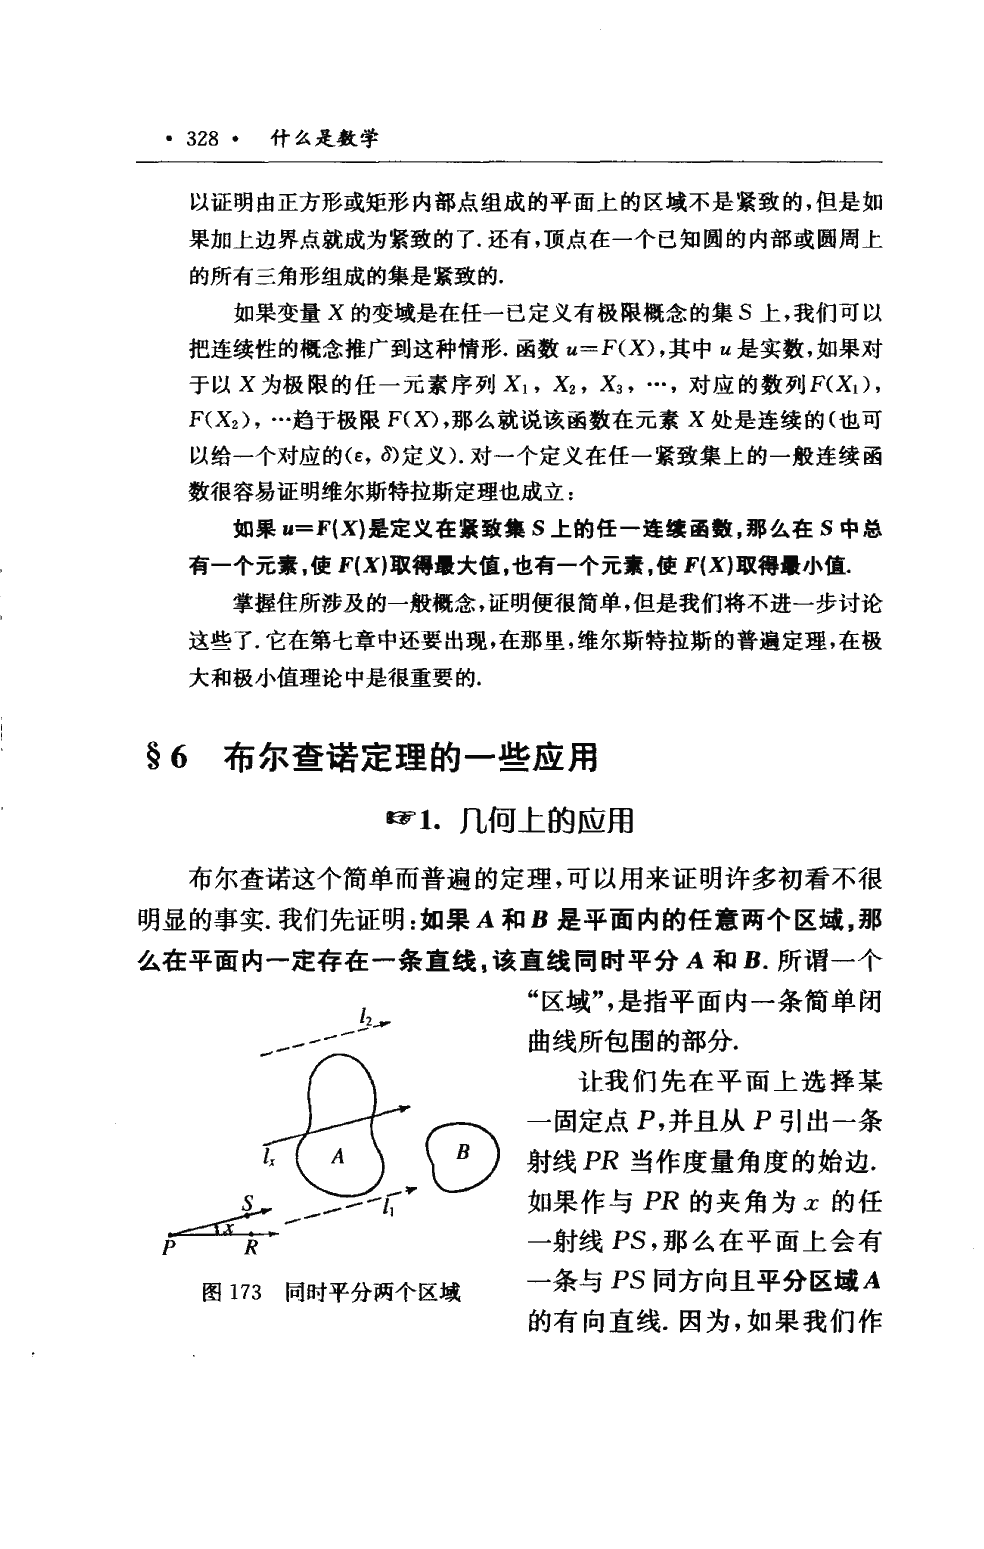
\includegraphics[height=1\textheight]{F:/life/2018AutumnTA/Exercises/4/intermediate-value-theorem1.png}
\end{center}
\end{figure}
\begin{figure}[H]
\begin{center}
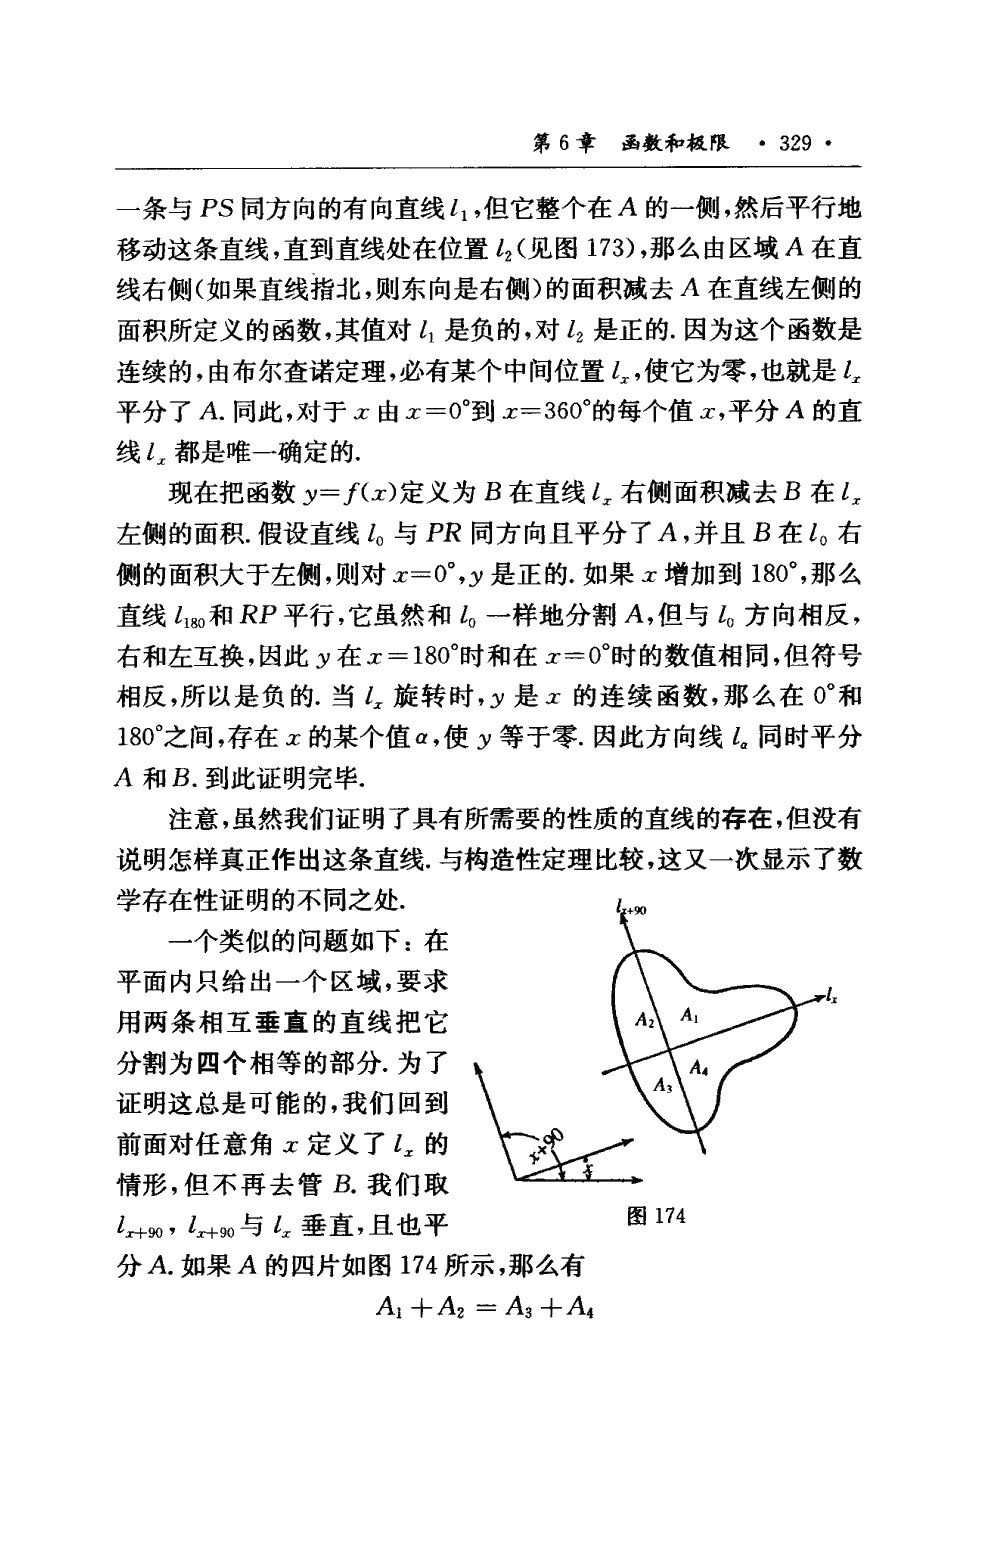
\includegraphics[height=1\textheight]{F:/life/2018AutumnTA/Exercises/4/intermediate-value-theorem2.png}
\end{center}
\end{figure}
\begin{figure}[H]
\begin{center}
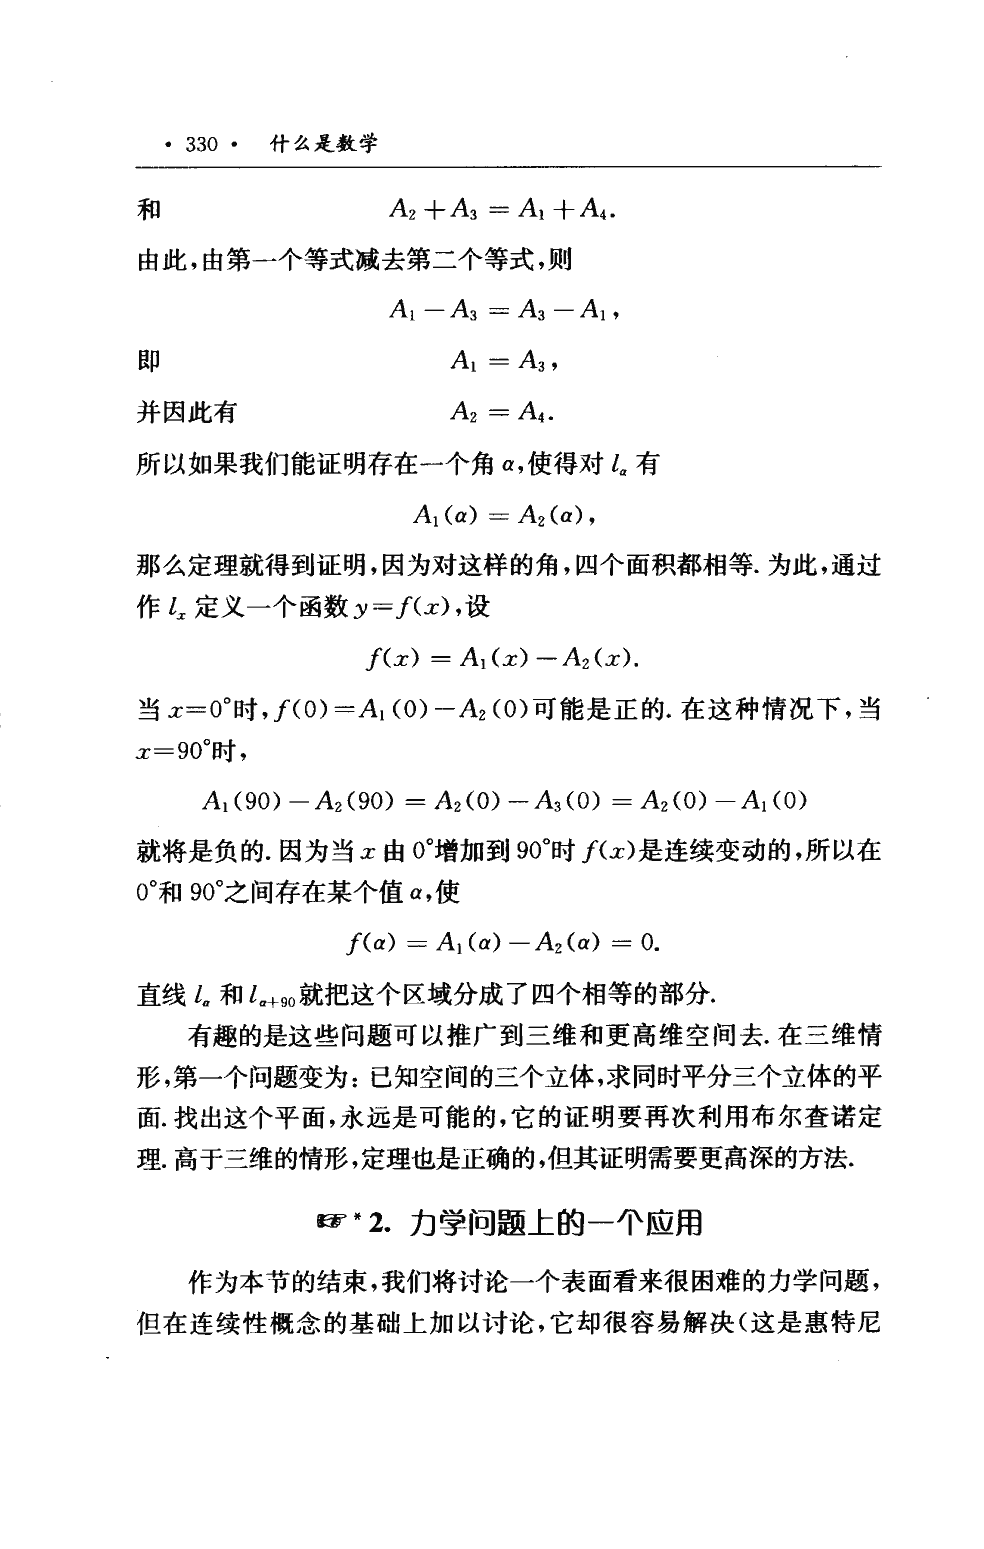
\includegraphics[height=1\textheight]{F:/life/2018AutumnTA/Exercises/4/intermediate-value-theorem3.png}
\end{center}
\end{figure}
\subsection{附录2}
\begin{figure}[H]
\begin{center}
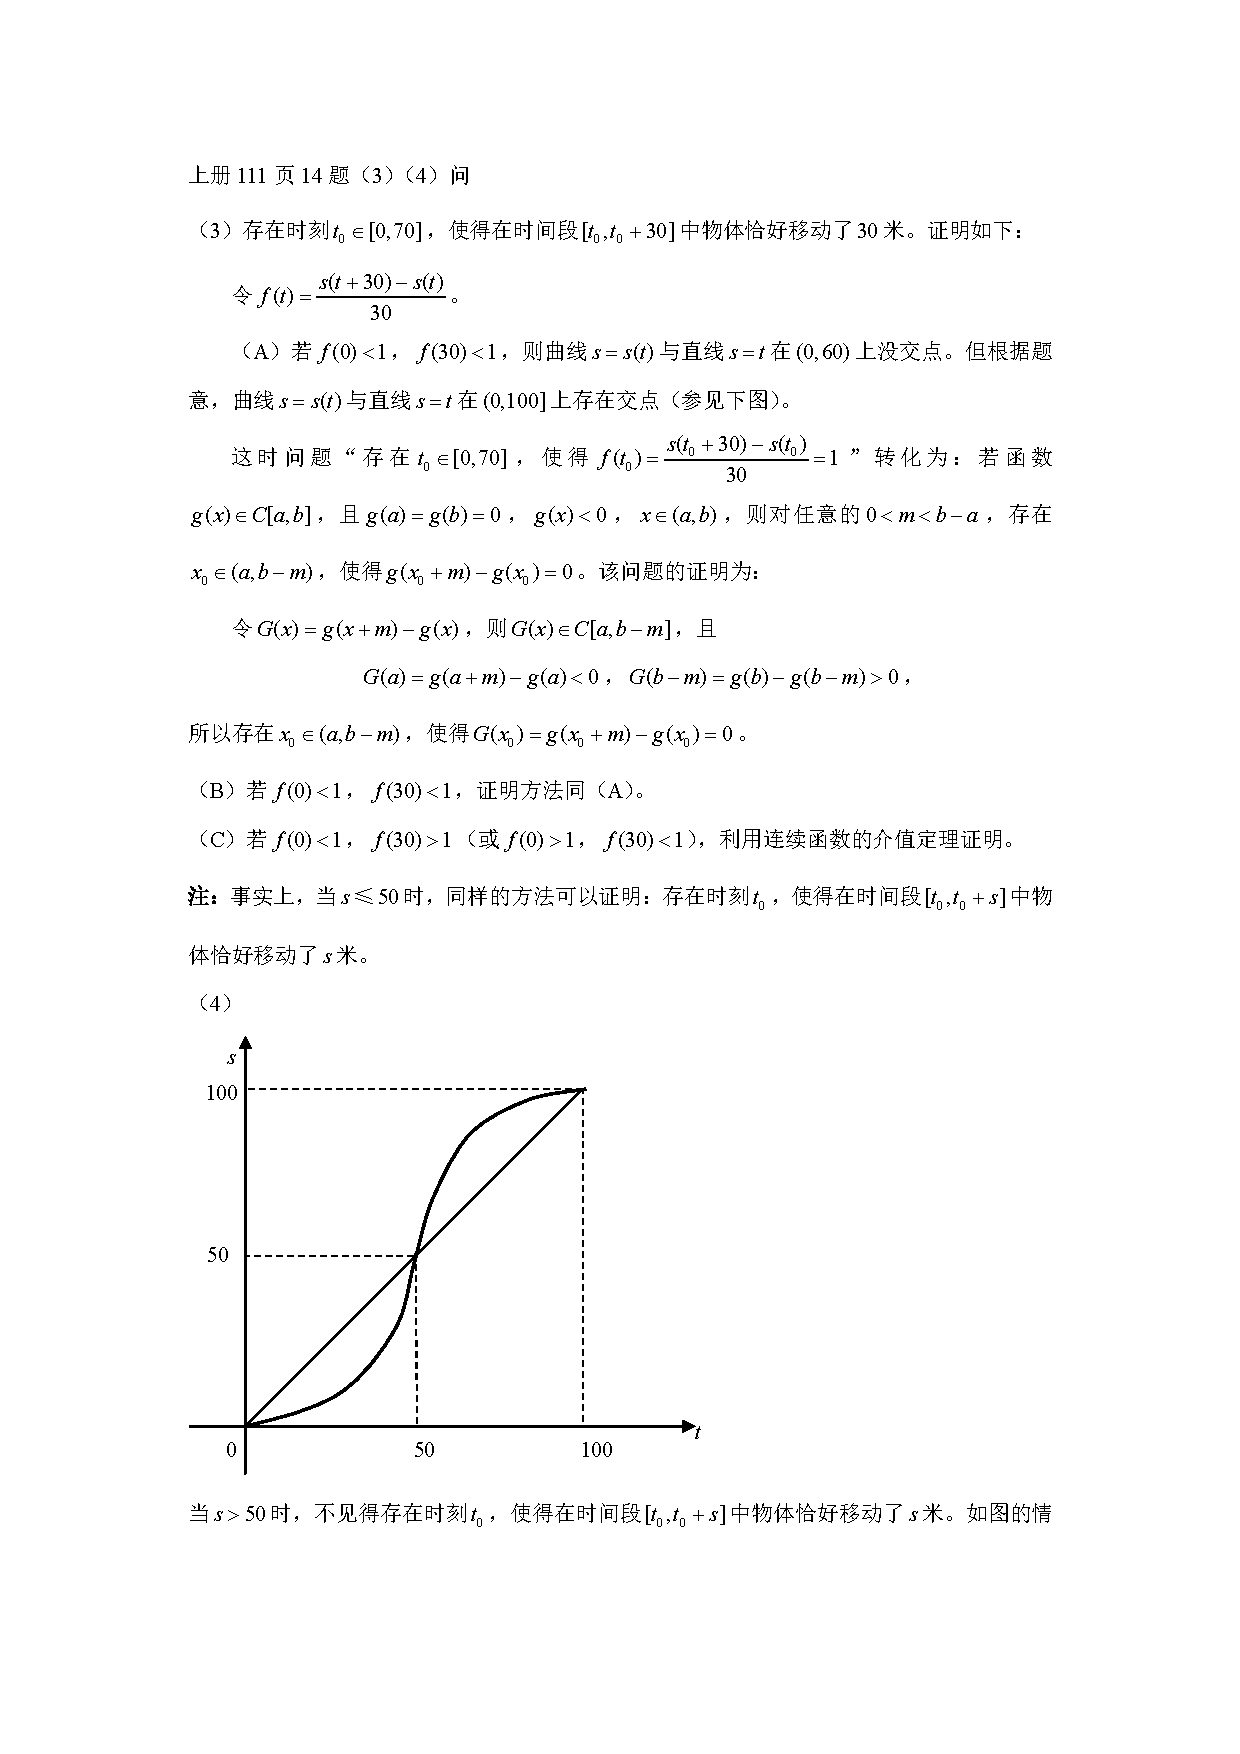
\includegraphics[height=1\textheight]{F:/life/2018AutumnTA/Exercises/4/Exercises.pdf}
\end{center}
\end{figure}
\begin{figure}[H]
\begin{center}
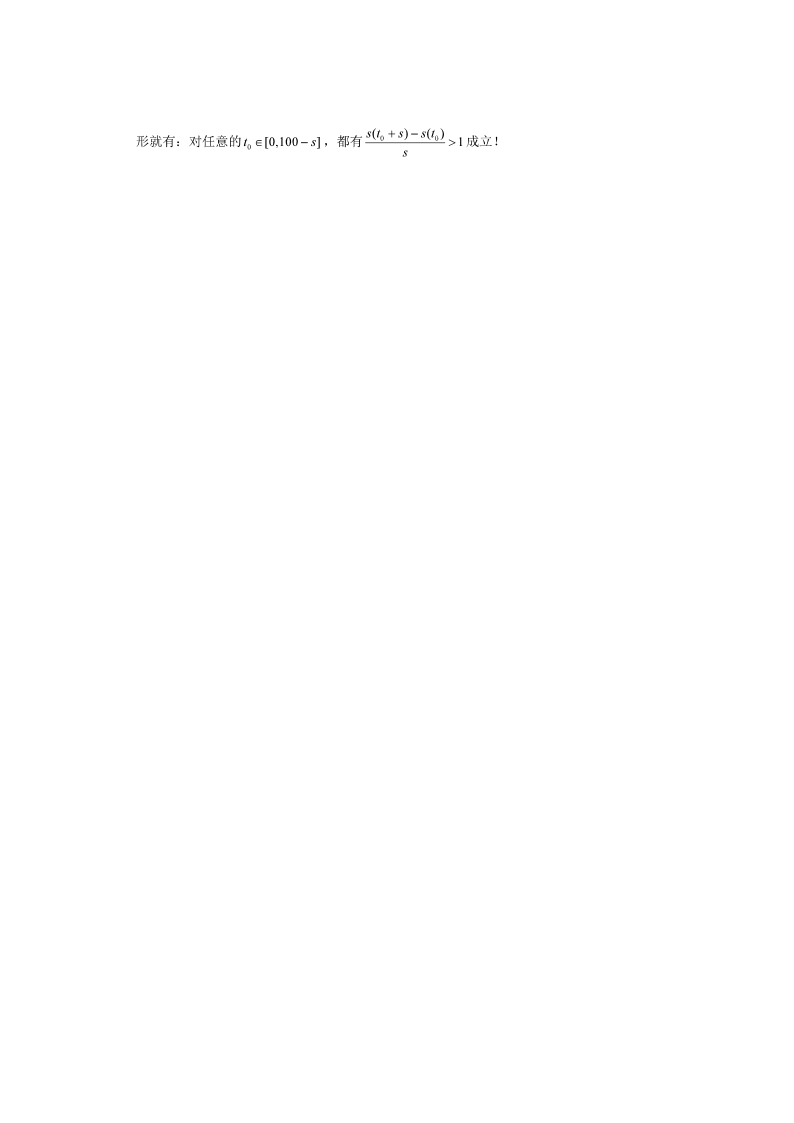
\includegraphics[height=1\textheight]{F:/life/2018AutumnTA/Exercises/4/Exercise2.png}
\end{center}
\end{figure}
\end{document}